
\noindent\begin{minipage}{\textwidth}
    \begin{table}[H]
        \centering
        \caption{Hiperparâmetros e Resultados do Melhor Modelo - vit\_v10\_BR\_opt\_aug}
        \vspace{0.2cm}
        \resizebox{\textwidth}{!}{%
            \begin{tabular}{ll | lrrr}
                \hline
                \multicolumn{2}{c|}{\textbf{Hiperparâmetros}} & \multicolumn{4}{c}{\textbf{Métricas por Classe}} \\ \hline
                \textbf{Parâmetro} & \textbf{Valor} & \textbf{Classe} & \textbf{Precisão} & \textbf{Recall} & \textbf{F1-Score} \\ \hline
    Agendador (Patience) & 3 & 31.2 & 0.6129 & 0.6847 & 0.6468 \\ 
Agendador de LR & ReduceLROnPlateau & 31.3 & 0.4966 & 0.3883 & 0.4358 \\ 
Architecture & vit\_b\_16 & 31.4 & 0.4281 & 0.5482 & 0.4808 \\ 
Augmentation (Método) & None & 32.3 & 0.5752 & 0.6878 & 0.6265 \\ 
Batch Size & 32 & 32.4 & 0.5357 & 0.4167 & 0.4688 \\ 
Decaimento de Peso (WD) & 0.0244 & 33.3 & 0.6232 & 0.5972 & 0.6099 \\ 
Dropout & 0.2083 & 41.4 & 0.4857 & 0.3617 & 0.4146 \\ 
Função de Perda & CrossEntropyLoss & 41.5 & 0.7600 & 0.4419 & 0.5588 \\ 
Hidden Units & 256 & 42.4 & 0.7586 & 0.3607 & 0.4889 \\ 
Label Smoothing & 0.0290 & 44.4 & 0.9200 & 0.7188 & 0.8070 \\ 
\cline{3-6} 
Otimizador & AdamW & \textbf{Média (Macro)} & 0.6196 & 0.5206 & 0.5538 \\ 
Taxa de Aprendizado (LR) & 2.61e-05 & \textbf{MCC} & \multicolumn{3}{c}{0.4809} \\ 
Unfreeze Layers & 4 &  & & &  \\ 
            \hline
            \end{tabular}%
        }
    \end{table}

    \begin{figure}[H]
        \centering
        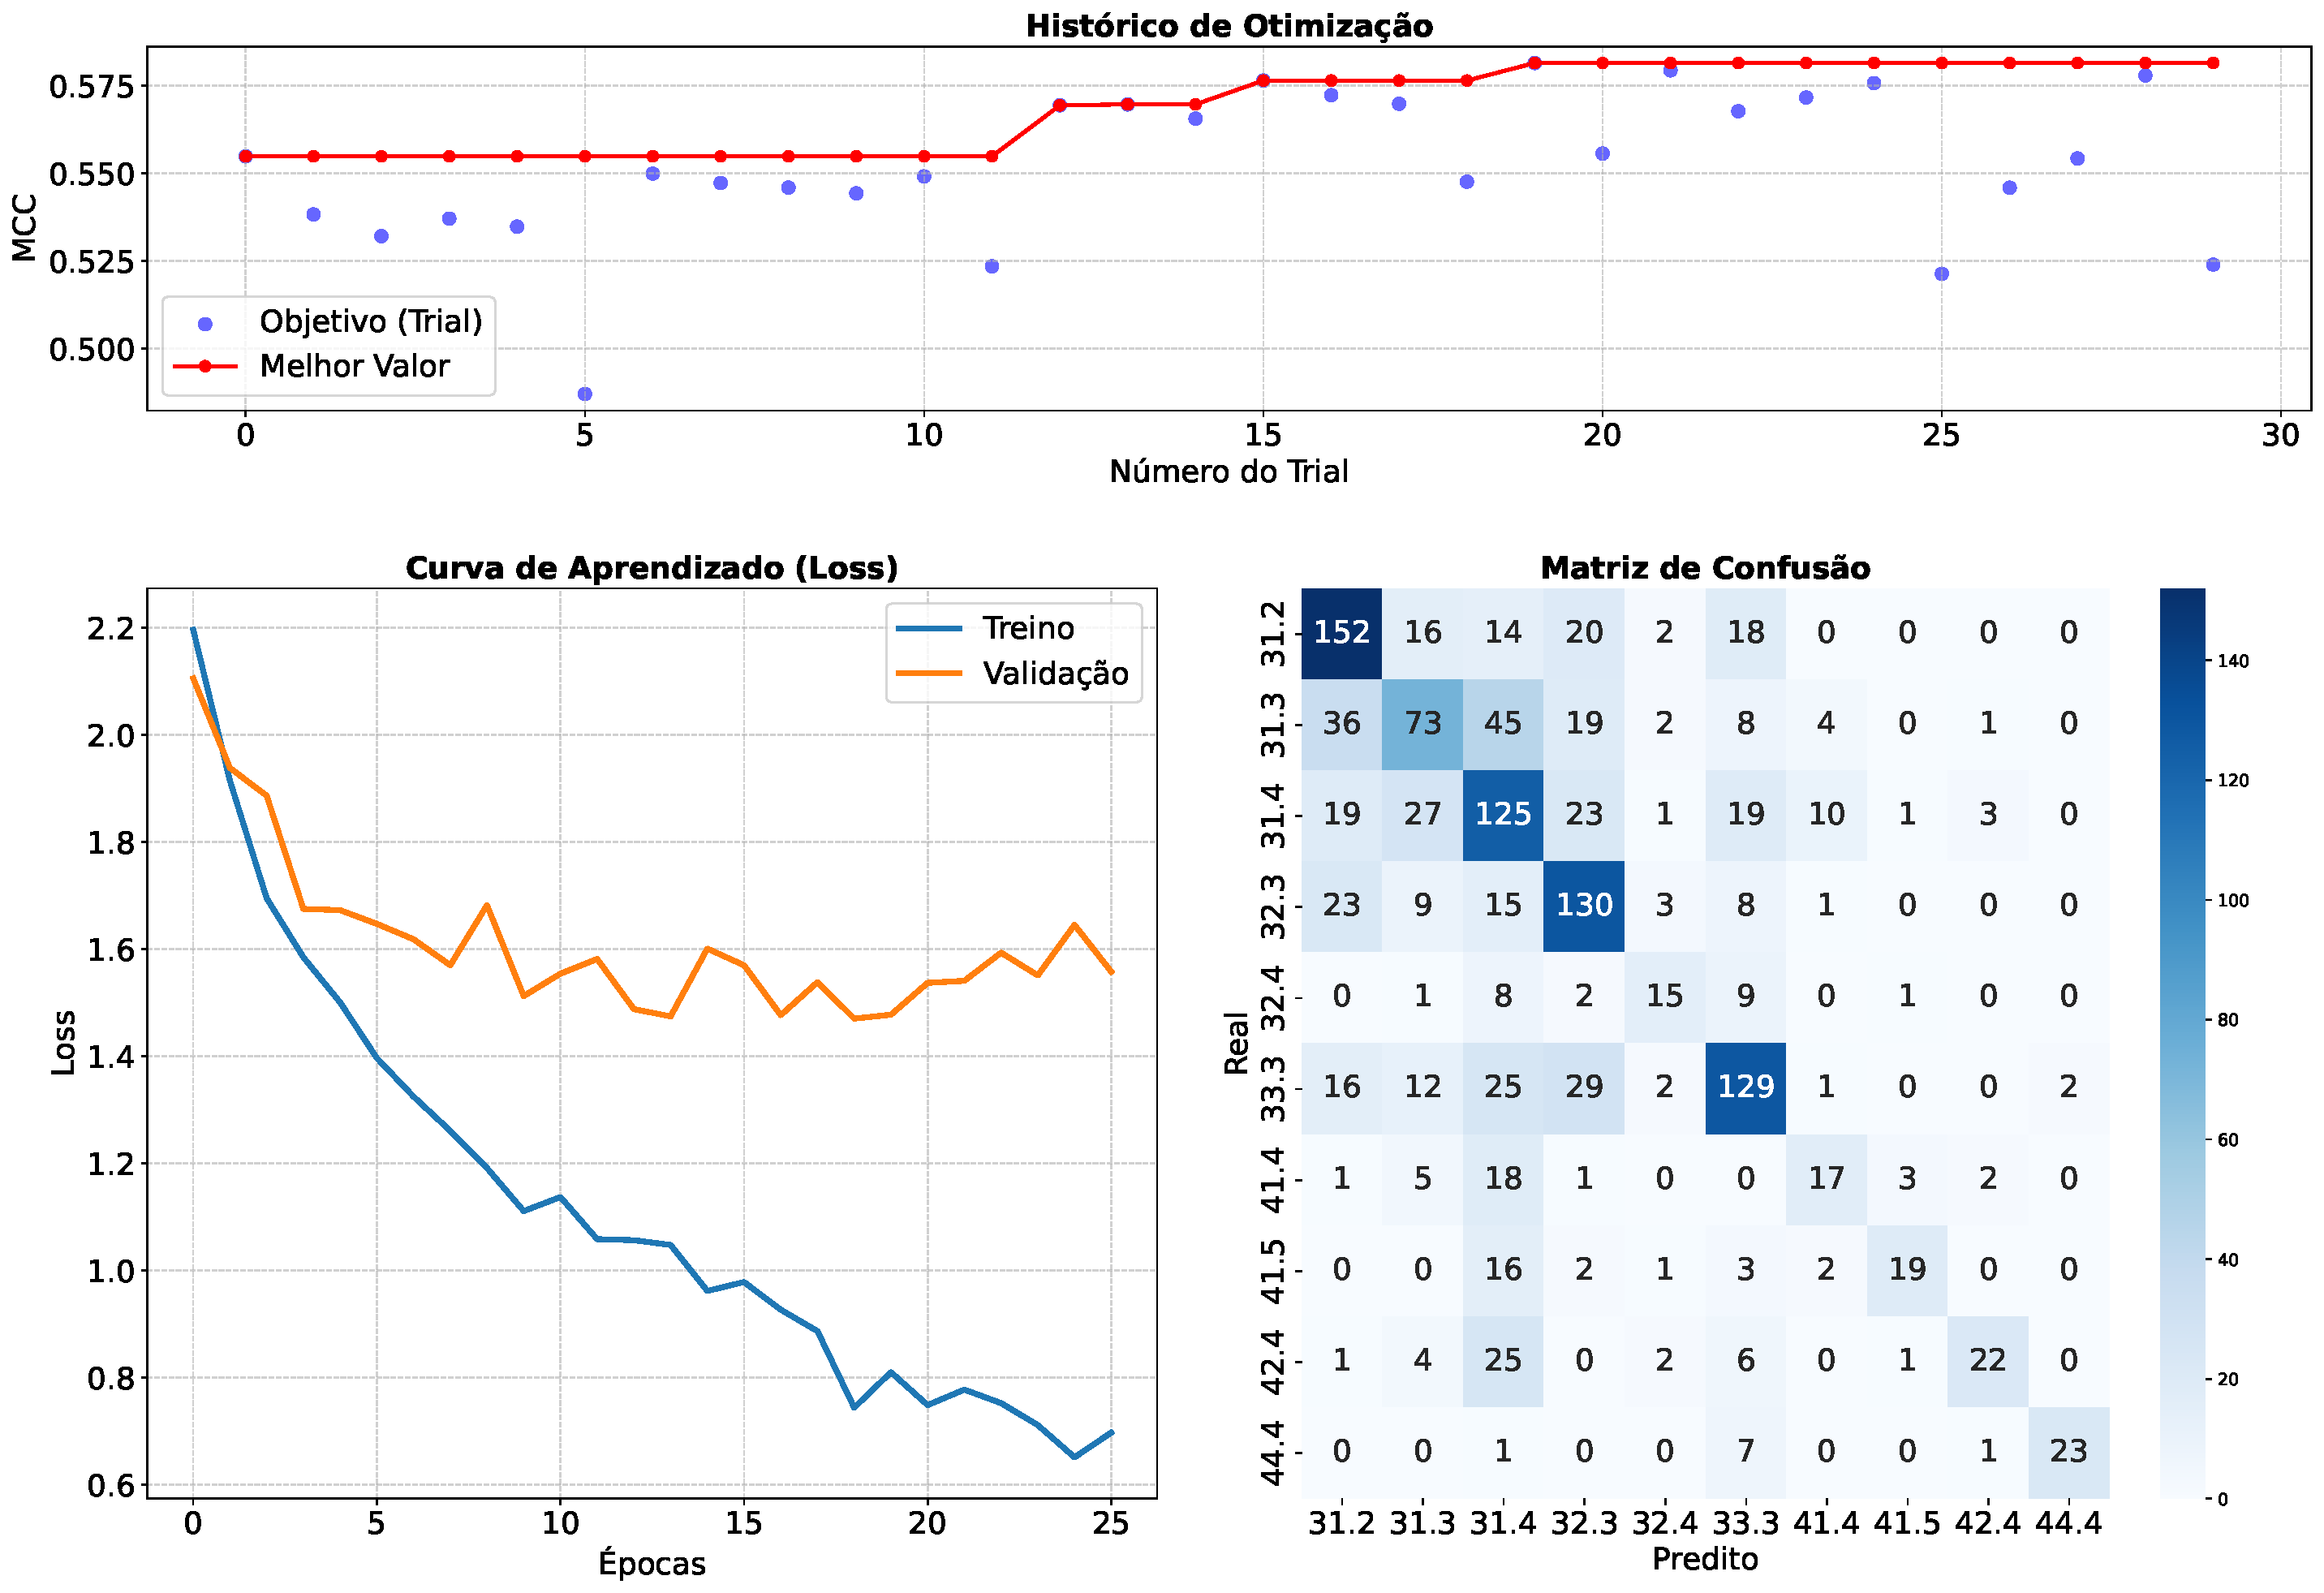
\includegraphics[width=0.85\textwidth]{tex/appendix/experiments/vit_v10_BR_opt_aug/dashboard_consolidado.pdf}
        \caption{Histórico de Otimização, Curvas de Aprendizado e Matriz de Confusão - vit\_v10\_BR\_opt\_aug}
    \end{figure}
\end{minipage}
\clearpage
